%%%%%%%%%%%%%%%%%%%%%%%%%%%%%%%%%%%%%%%%%%%%%%%%%%%%%%%%%%%%%%%%%%%%%%%%%%%%%%%%
%
% https://www.sharelatex.com/learn/Beamer
%
%%%%%%%%%% 
\documentclass{beamer}
	\usetheme{ACUAS}
%	\usetheme{Madrid}
%
% 	- Hiding the presentation controls in LaTeX beamer presentation [closed]
%		- https://stackoverflow.com/questions/3017030/hiding-the-presentation-controls-in-latex-beamer-presentation
%	\usetheme{Dresden}
%		\usecolortheme{beaver}
	\setbeamertemplate{navigation symbols}{}
	%
	% Gitterllinien auf den Folien anzeigen
	%
	%\beamertemplategridbackground[1cm]


%%%%%%%%%%%%%%%%%%%%%%%%%%%%%%%%%%%%%%%%%%%%%%%%%%%%%%%%%%%%%%%%%%%%%%%%%%%%%%%%
%
% Packages
%
%%%%%%%%%% 
\usepackage{fontspec}
\usepackage{lmodern}
\usepackage{polyglossia}
	\setmainlanguage[variant=german, spelling=new]{german}
\usepackage{graphicx}
	\graphicspath{{./logos/}{./bilder/}}

%
% bibtex vs. biber and biblatex vs. natbib
%	- https://tex.stackexchange.com/questions/25701/bibtex-vs-biber-and-biblatex-vs-natbib
% The biblatex Package - Programmable Bibliographies and Citations
% 	- http://ftp.math.purdue.edu/mirrors/ctan.org/macros/latex/exptl/biblatex/doc/biblatex.pdf
% Biblatex citation order
%	- https://tex.stackexchange.com/questions/51434/biblatex-citation-order
% 		- sorting=ydnt: Sort by year (descending), name, title.
%		- sorting=none: Do not sort at all. All entries are processed in citation order.
%
%\usepackage[
%	backend=biber,
%	style=numeric-comp,
%	%style=ieee,
%	sorting=none,
%]{biblatex}
%	\addbibresource{quellen.bib}
	
%\usepackage{showframe}

\usepackage[mode=text]{siunitx}
	\sisetup{locale=DE, range-phrase=--, product-units=single, binary-units=true}
	\DeclareSIUnit{\mAh}{mAh}
	\DeclareSIUnit{\belmilliwatt}{Bm}
	\DeclareSIUnit{\dBm}{\deci\belmilliwatt}
	
\usepackage{subcaption}
	% How to remove figure caption prefix “figure” in beamer
	% https://tex.stackexchange.com/questions/82456/how-to-remove-figure-caption-prefix-figure-in-beamer
	\captionsetup[figure]{labelformat=empty, font=scriptsize, skip=2pt}

\usepackage{tikz}
	\usetikzlibrary{trees,graphs,shapes,mindmap}
	\tikzstyle{node_normal} = [circle, draw, inner sep=0pt, minimum size=20pt]
	\tikzstyle{node_deleted} = [circle, draw, dashed, inner sep=0pt, minimum size=20pt]
	\tikzstyle{node_bold} = [circle, draw, ultra thick, inner sep=0pt, minimum size=20pt]
	\tikzstyle{edge_deleted} = [dashed]
	\tikzstyle{edge_hamilton} = [ultra thick]
	\tikzstyle{edge_normal} = []

\usepackage{tikzducks}


%%%%%%%%%%%%%%%%%%%%%%%%%%%%%%%%%%%%%%%%%%%%%%%%%%%%%%%%%%%%%%%%%%%%%%%%%%%%%%%%
%
% Information to be included in the title page
%
%%%%%%%%%%
\title[Hamiltonsche Grafen und das TSP]{Hamiltonsche Graphen und das\\ Traveling Salesman Problem (TSP)}
\subtitle{Mathematische Methoden der Informatik}
\author[]
{
	Albert Kasdorf, Andreas Janster, Alex Bibanaev, Georg Braun
}
\institute[FH Aachen]
{
	FH Aachen\\
	Fachbereich Elektrotechnik und Informationstechnik\\
	Ingenieur-Informatik
}
\date{09.05.2018}

\newtheorem{mydef}{Definition}
\newtheorem{mylem}{Lemma}
\newtheorem{mysat}{Satz}

\newcommand\blfootnote[1]{%
	\begingroup
	\renewcommand\thefootnote{}\footnote{#1}%
	\addtocounter{footnote}{-1}%
	\endgroup
}


\begin{document}


%%%%%%%%%%%%%%%%%%%%%%%%%%%%%%%%%%%%%%%%%%%%%%%%%%%%%%%%%%%%%%%%%%%%%%%%%%%%%%%%
%
% Titelseite
%
%%%%%%%%%%
\frame{\titlepage}


%%%%%%%%%%%%%%%%%%%%%%%%%%%%%%%%%%%%%%%%%%%%%%%%%%%%%%%%%%%%%%%%%%%%%%%%%%%%%%%%
%
% Inhaltsverzeichnis?
%
%%%%%%%%%%
\begin{frame}{Inhalt}
%\tableofcontents

%\begin{itemize}
%	\item Hamiltonsche Graphen (Albert)
%	\item Traveling Salesman Problem (Andreas \& Alex)
%	\item Algorithmen (Georg)
%\end{itemize}

%\begin{center}
	\begin{tabular}{ l r }
		Hamiltonsche Graphen & (Albert) \\
		\\
		Traveling Salesman Problem & (Andreas \& Alex) \\
		\\
		Algorithmen & (Georg)
	\end{tabular}
%\end{center}

\end{frame}


%%%%%%%%%%%%%%%%%%%%%%%%%%%%%%%%%%%%%%%%%%%%%%%%%%%%%%%%%%%%%%%%%%%%%%%%%%%%%%%%
%
%
%
%%%%%%%%%%
\part{Hamiltonsche Graphen}


%%%%%%%%%%%%%%%%%%%%%%%%%%%%%%%%%%%%%%%%%%%%%%%%%%%%%%%%%%%%%%%%%%%%%%%%%%%%%%%%
%
%
%
%%%%%%%%%%
\begin{frame}{Hamiltonsche Graphen\\\normalsize{Motivation}}
\only<1>
{
	\begin{itemize}
		\item Bernd und Anna planen ihre Hochzeit.
	\end{itemize}
	\begin{figure}
		\centering
		
\includegraphics[width=0.5\textwidth]{bernd_und_anna.jpg}
	\end{figure}
	\blfootnote{\tiny{Bildquelle: \url{https://gamesageddon.com/stock/media?id=28098782}}}
}
\only<2>
{
	\begin{itemize}
		\item Beim Hochzeitsessen soll jeder Gast zwischen zwei Ihm bekannten Personen sitzen.
	\end{itemize}
	\begin{figure}
		\centering
		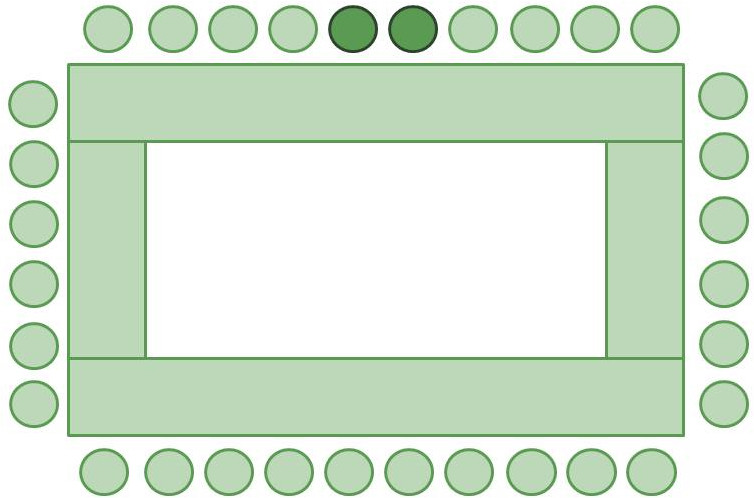
\includegraphics[width=0.5\textwidth]{tischform.jpg}
	\end{figure}
	\blfootnote{\tiny{Bildquelle: \url{http://www.hochzeit-perfekt-geplant.de/artikel/planung/tischordnung-hochzeit.html}}}
}
\only<3>
{
	\begin{itemize}
		\item Auf dem Junggesellenabschied mit seinen alten Studienkollegen kommt Bernd eine Idee.
	\end{itemize}
	\begin{figure}
		\centering
		
\includegraphics[width=0.5\linewidth]{junggesellenabschied.jpg}
	\end{figure}
	\blfootnote{\tiny{Bildquelle: \url{https://de.depositphotos.com/168789924}}}
}
\only<4>
{
	\begin{itemize}
		\item Auf einem Bierdeckel zeichnet Bernd einen Graphen, der die Bekanntschaft zwischen den Hochzeitsgästen modelliert.
	\end{itemize}
	\begin{figure}
		\centering
		\begin{tikzpicture}[scale=0.6]
			\node (A) at (-1,+0) [node_bold] {a};
			\node (B) at (+1,+0) [node_bold] {b};
			\node (C) at (-4,+0) [node_normal] {c};
			\node (D) at (-4,-3) [node_normal] {d};
			\node (E) at (-4,+4) [node_normal] {e};
			\node (F) at (-6,+2) [node_normal] {f};
			\node (G) at (+0,+2) [node_normal] {g};
			\node (H) at (+4,+4) [node_normal] {h};
			\node (I) at (+4,+0) [node_normal] {i};
			\node (J) at (+2,-3) [node_normal] {j};
			
			\draw[edge_normal] (A)--(B) (A)--(C) (A)--(D) (A)--(E) (A)--(F) (A)--(G);
			\draw[edge_normal] (B)--(D) (B)--(I) (B)--(J) (B)--(G) (B)--(H);
			\draw[edge_normal] (C)--(D) (C)--(F);
			\draw[edge_normal] (D)--(F);
			\draw[edge_normal] (E)--(F) (E)--(G) (E)--(H);
			\draw[edge_normal] (F)--(G);
			\draw[edge_normal] (G)--(H) (G)--(I);
			\draw[edge_normal] (I)--(J);
		\end{tikzpicture}
	\end{figure}
}
\only<5>
{
	\begin{itemize}
		\item Wenn in dem Graphen ein Kreis gefunden wird, der jeden Gast genau einmal enthält, dann kann jeder Gast neben zwei Ihm bekannten Gästen sitzen.
	\end{itemize}
	\begin{figure}
		\centering
		\begin{tikzpicture}[scale=0.6]
			\node (A) at (-1,+0) [node_bold] {a};
			\node (B) at (+1,+0) [node_bold] {b};
			\node (C) at (-4,+0) [node_normal] {c};
			\node (D) at (-4,-3) [node_normal] {d};
			\node (E) at (-4,+4) [node_normal] {e};
			\node (F) at (-6,+2) [node_normal] {f};
			\node (G) at (+0,+2) [node_normal] {g};
			\node (H) at (+4,+4) [node_normal] {h};
			\node (I) at (+4,+0) [node_normal] {i};
			\node (J) at (+2,-3) [node_normal] {j};
			
			\draw[edge_normal] (A)--(B) (A)--(C) (A)--(D) (A)--(E) (A)--(F) (A)--(G);
			\draw[edge_normal] (B)--(D) (B)--(I) (B)--(J) (B)--(G) (B)--(H);
			\draw[edge_normal] (C)--(D) (C)--(F);
			\draw[edge_normal] (D)--(F);
			\draw[edge_normal] (E)--(F) (E)--(G) (E)--(H);
			\draw[edge_normal] (F)--(G);
			\draw[edge_normal] (G)--(H) (G)--(I);
			\draw[edge_normal] (I)--(J);
			
			\draw[edge_hamilton] (A)--(B)--(J)--(I)--(G)--(H)--(E)--(F)--(C)--(D)--(A);
		\end{tikzpicture}
	\end{figure}
}
\end{frame}


%%%%%%%%%%%%%%%%%%%%%%%%%%%%%%%%%%%%%%%%%%%%%%%%%%%%%%%%%%%%%%%%%%%%%%%%%%%%%%%%
%
%
%
%%%%%%%%%%
\begin{frame}{Hamiltonsche Graphen\\\normalsize{Definition}}

\begin{columns}
	\column{0.5\linewidth}
	\begin{block}{Definition:}
		Ein Graph heißt \textbf{hamiltonsch} oder \textbf{Hamilton-Graph}, wenn in ihm ein Kreis existiert, der jeden Knoten genau einmal enthält. Ein solcher Kreis heißt auch \textbf{Hamilton-Kreis}.
	\end{block}
	\column{0.5\linewidth}
	\begin{figure}
%		\begin{tikzpicture}
%			\node (A) at (+0,+1) [node_normal] {a};
%			\node (B) at (+0,-0.2) [node_normal] {b};
%			\node (C) at (-1,-1) [node_normal] {c};
%			\node (D) at (+1,-1) [node_normal] {d};
%	
%			\draw (A)--(C) (C)--(D) (D)--(A);
%			\draw (B)--(A) (B)--(C) (B)--(D);
%	
%			\draw[black, ultra thick] (A)--(C)--(B)--(D)--(A);
%		\end{tikzpicture}
		\begin{tikzpicture}
			\def\inc{((2*pi)/5)+pi/2}
			\def\ro{2.1}
			\node (A) at ({cos(deg(0*\inc))*\ro}, {sin(deg(0*\inc))*\ro}) [node_normal] {a};
			\node (B) at ({cos(deg(1*\inc))*\ro}, {sin(deg(1*\inc))*\ro}) [node_normal] {b};
			\node (C) at ({cos(deg(2*\inc))*\ro}, {sin(deg(2*\inc))*\ro}) [node_normal] {c};
			\node (D) at ({cos(deg(3*\inc))*\ro}, {sin(deg(3*\inc))*\ro}) [node_normal] {d};
			\node (E) at ({cos(deg(4*\inc))*\ro}, {sin(deg(4*\inc))*\ro}) [node_normal] {e};

			\draw[edge_normal] (A)--(B)--(C)--(D)--(E)--(A);
			\draw[edge_hamilton] (A)--(C)--(E)--(B)--(D)--(A);

			\begin{scope}[xshift=-10pt, scale=.3, yshift=-30pt]
				\duck[graduate=gray!20!black,tassel=red!70!black]
			\end{scope}
		\end{tikzpicture}
	\end{figure}
\end{columns}

\end{frame}


%%%%%%%%%%%%%%%%%%%%%%%%%%%%%%%%%%%%%%%%%%%%%%%%%%%%%%%%%%%%%%%%%%%%%%%%%%%%%%%%
%
% 
%
%%%%%%%%%%
\begin{frame}{Hamiltonsche Graphen\\\normalsize{Übung}}
\begin{block}{Aufgabe:}
	Untersuchen Sie die Graphen auf dem Übungsblatt anhand der folgenden Kriterien.
\end{block}
\begin{itemize}
	\item Eulersch / Hamiltonsch
	\item Knotengrad
	\begin{itemize}
		\item Minimal / Maximal
		\item Baum
		\item Kreisfrei
	\end{itemize}
	\item Zusammenhang
	\item ?Multigraph?
	\begin{itemize}
		\item Parallele Kanten
		\item Schleifen
	\end{itemize}
\end{itemize}
%\begin{figure}
%\begin{tikzpicture}[
%	mindmap,
%	grow cyclic,
%	every node/.style=concept,
%	concept color=orange!100,
%	level 1/.append style={sibling angle=90},
%	level 2/.append style={sibling angle=45}
%]
%\node{Hamilton-\\ Graph}
%	child{node{Multigrad}
%		child{node{Parallele Kanten}}
%		child{node{Schleifen}}
%	}
%	child{node{Knotengrad}
%		child{node{Minimal}}
%		child{node{Maximal}}
%		child{node{Baum}}
%		child{node{Kreisfrei}}
%	}
%	child{node{Zusammenhang}}
%	child{node{Eulersch}};
%\end{tikzpicture}
%\end{figure}
\end{frame}


%%%%%%%%%%%%%%%%%%%%%%%%%%%%%%%%%%%%%%%%%%%%%%%%%%%%%%%%%%%%%%%%%%%%%%%%%%%%%%%%
%
%
%
%%%%%%%%%%
\begin{frame}{Hamiltonsche Graphen\\\normalsize{Vollständigkeit}}

\begin{columns}

\column{0.5\linewidth}
\begin{block}{Definition:}
Ein Graph $G=(V,E)$ heißt \textbf{vollständig}, wenn jeder Knoten zu jedem anderen Knoten benachbart ist. Da der Graph also nur von der Anzahl der Knoten $n$ abhängt, bezeichnet man ihn auch als $K_n$.
\end{block}

\column{0.5\linewidth}
\begin{figure}
\centering
\begin{tikzpicture}
\node (A) at (0,0) [node_normal] {a};
\node (B) at (0,2) [node_normal] {b};
\node (C) at (2,2) [node_normal] {c};
\node (D) at (2,0) [node_normal] {d};

\draw[edge_normal] (A)--(C) (C)--(D) (D)--(A);
\draw[edge_normal] (B)--(A) (B)--(C) (B)--(D);

\draw[edge_hamilton] (A)--(C)--(B)--(D)--(A);
\end{tikzpicture}
\caption{$K_4$}
\end{figure}

\end{columns}

\end{frame}


%%%%%%%%%%%%%%%%%%%%%%%%%%%%%%%%%%%%%%%%%%%%%%%%%%%%%%%%%%%%%%%%%%%%%%%%%%%%%%%%
%
%
%
%%%%%%%%%%
\begin{frame}{Hamiltonsche Graphen\\\normalsize{Minimalgrad}}

\begin{columns}

\column{0.5\linewidth}
%\begin{block}{Definition:}
%Sei $G=(V,E)$ ein Graph. Der Wert $\delta(G)$ gibt den \textbf{Minimalgrad} in $G$ an, d.h. die kleinste in $G$ vorkommende Gradzahl, und $\Delta(G)$ den \textbf{Maximalgrad} eines Knoten in G, d.h. die größte in $G$ vorkommende Gradzahl.
%\end{block}

\begin{block}{Lemma:}
	Ein hamiltonscher Graph enthält keinen Knoten mit Grad 1.
\end{block}

\column{0.5\linewidth}
\begin{figure}
\centering
\begin{tikzpicture}
\node (A) at (0,0) [node_normal] {a};
\node (B) at (0,2) [node_normal] {b};
\node (C) at (1,1) [node_normal] {c};
\node (D) at (2,1) [node_normal] {d};
\draw[edge_normal] (A)--(B)--(C)--(D);
\draw[edge_normal] (A)--(C);
\end{tikzpicture}
\end{figure}

\end{columns}

\end{frame}


%%%%%%%%%%%%%%%%%%%%%%%%%%%%%%%%%%%%%%%%%%%%%%%%%%%%%%%%%%%%%%%%%%%%%%%%%%%%%%%%
%
%
%
%%%%%%%%%%
\begin{frame}{Hamiltonsche Graphen\\\normalsize{Satz von Dirac (1/2)}}
\begin{columns}
\column{0.5\linewidth}
\begin{block}{Definition:}
Sei $G=(V,E)$ ein Graph. Der Wert $\delta(G)$ gibt den \textbf{Minimalgrad} in $G$ an, d.h. die kleinste in $G$ vorkommende Gradzahl, und $\Delta(G)$ den \textbf{Maximalgrad} eines Knoten in G, d.h. die größte in $G$ vorkommende Gradzahl.
\end{block}
\column{0.5\linewidth}
\begin{figure}
\centering
\captionsetup{justification=centering}
\begin{tikzpicture}
\node (A) at (0,0) [node_normal] {a};
\node (B) at (0,2) [node_normal] {b};
\node (C) at (1,3) [node_normal] {c};
\node (D) at (2,2) [node_normal] {d};
\node (E) at (2,0) [node_normal] {e};
\node (F) at (1,1) [node_normal] {f};
\draw[edge_normal] (A)--(B) (A)--(F) (A)--(E);
\draw[edge_normal] (B)--(C) (B)--(D) (B)--(F);
\draw[edge_normal] (D)--(C) (D)--(F) (D)--(E);
\draw[edge_normal] (E)--(F);
\end{tikzpicture}
\caption{$\delta(G)=2$\\ $\Delta(G)=4$}
\end{figure}
\end{columns}
\end{frame}


%%%%%%%%%%%%%%%%%%%%%%%%%%%%%%%%%%%%%%%%%%%%%%%%%%%%%%%%%%%%%%%%%%%%%%%%%%%%%%%%
%
%
%
%%%%%%%%%%
\begin{frame}{Hamiltonsche Graphen\\\normalsize{Satz von Dirac (2/2)}}
\begin{columns}
\column{0.5\linewidth}
\begin{block}{Satz von Dirac:}
Sei G ein einfacher Graph mit mindestens drei Knoten, für den außerdem $\delta(G)\geq 0.5\cdot n$ gilt. Dann enthält der Graph einen Hamilton-Kreis.
\end{block}
\only<3>
{
	\begin{block}{}
		Es gibt auch Graphen die den Satz von Dirac nicht erfüllen und trotzdem einen Hamilton-Kreis besitzen.
	\end{block}
}
\column{0.5\linewidth}
\only<2>
{
\begin{figure}
\centering
\begin{tikzpicture}
\def\inc{((2*pi)/5)+pi/2}
\def\ro{2.1}
\node (A) at (0,0) [node_normal] {a};
\node (B) at ({cos(deg(0*\inc))*\ro}, {sin(deg(0*\inc))*\ro}) [node_normal] {b};
\node (C) at ({cos(deg(1*\inc))*\ro}, {sin(deg(1*\inc))*\ro}) [node_normal] {c};
\node (D) at ({cos(deg(2*\inc))*\ro}, {sin(deg(2*\inc))*\ro}) [node_normal] {d};
\node (E) at ({cos(deg(3*\inc))*\ro}, {sin(deg(3*\inc))*\ro}) [node_normal] {e};
\node (F) at ({cos(deg(4*\inc))*\ro}, {sin(deg(4*\inc))*\ro}) [node_normal] {f};

\draw[edge_normal] (A)--(B) (A)--(C) (A)--(D) (A)--(E) (A)--(F);
\draw[edge_normal] (B)--(C)--(D)--(E)--(F)--(B);
\draw[edge_normal] (D)--(B) (D)--(F);
\draw[edge_hamilton] (D)--(B)--(C)--(A)--(F)--(E)--(D);
\end{tikzpicture}
\captionsetup{justification=centering}
\caption{$n=6$\\ $\delta(G)=3$}
\end{figure}
}
\only<3>
{
\begin{figure}
	\centering
	\begin{tikzpicture}
	\def\inc{((2*pi)/6)+pi/2}
	\def\ro{2.1}
	\node (A) at ({cos(deg(0*\inc))*\ro}, {sin(deg(0*\inc))*\ro}) [node_normal] {a};
	\node (B) at ({cos(deg(1*\inc))*\ro}, {sin(deg(1*\inc))*\ro}) [node_normal] {b};
	\node (C) at ({cos(deg(2*\inc))*\ro}, {sin(deg(2*\inc))*\ro}) [node_normal] {c};
	\node (D) at ({cos(deg(3*\inc))*\ro}, {sin(deg(3*\inc))*\ro}) [node_normal] {d};
	\node (E) at ({cos(deg(4*\inc))*\ro}, {sin(deg(4*\inc))*\ro}) [node_normal] {e};
	\node (F) at ({cos(deg(5*\inc))*\ro}, {sin(deg(5*\inc))*\ro}) [node_normal] {f};

	\draw[edge_hamilton] (A)--(B)--(C)--(D)--(E)--(F)--(A);
	\end{tikzpicture}
	\captionsetup{justification=centering}
	\caption{$n=6$\\ $\delta(G)=2$}
\end{figure}
}
\end{columns}
\end{frame}


%%%%%%%%%%%%%%%%%%%%%%%%%%%%%%%%%%%%%%%%%%%%%%%%%%%%%%%%%%%%%%%%%%%%%%%%%%%%%%%%
%
%
%
%%%%%%%%%%
\begin{frame}{Hamiltonsche Graphen\\\normalsize{Zusammenhang}}
\begin{columns}
\column{0.5\linewidth}
\begin{block}{Lemma:}
Falls ein Graph hamiltonsch ist, dann ist er auch zusammenhängend.
\end{block}
\column{0.5\linewidth}
\only<2>
{
\begin{figure}
\centering
\begin{tikzpicture}
\node (A) at (0,0) [node_normal] {a};
\node (B) at (1,1) [node_normal] {b};
\node (C) at (2,0) [node_normal] {c};
\node (D) at (0,3) [node_normal] {d};
\node (E) at (2,3) [node_normal] {e};
\node (F) at (1,2) [node_normal] {f};
\draw[edge_normal] (A)--(B)--(C)--(A);
\draw[edge_normal] (D)--(E)--(F)--(D);
\end{tikzpicture}
\captionsetup{justification=centering}
\caption{Ein nicht zusammenhängender Graph ist auch nicht hamiltonsch.}
\end{figure}
}
\end{columns}
\end{frame}


%%%%%%%%%%%%%%%%%%%%%%%%%%%%%%%%%%%%%%%%%%%%%%%%%%%%%%%%%%%%%%%%%%%%%%%%%%%%%%%%
%
%
%
%%%%%%%%%%
\begin{frame}{Hamiltonsche Graphen\\\normalsize{Zusammenhangskomponenten}}
\begin{columns}
\column{0.5\linewidth}
\begin{block}{Satz:}
Für jeden hamiltonschen Graphen gilt: Wenn $k$ Knoten aus dem Graphen gelöscht werden, zerfällt der Graph in höchstens $k$ Zusammenhangskomponenten.
\end{block}
\column{0.5\linewidth}
\only<2>
{
\begin{figure}
\centering
\begin{tikzpicture}
\def\inc{((2*pi)/6)+pi/2}
\def\ro{2.1}
\node (A) at ({cos(deg(0*\inc))*\ro}, {sin(deg(0*\inc))*\ro}) [node_normal] {a};
\node (B) at ({cos(deg(1*\inc))*\ro}, {sin(deg(1*\inc))*\ro}) [node_normal] {b};
\node (C) at ({cos(deg(2*\inc))*\ro}, {sin(deg(2*\inc))*\ro}) [node_normal] {c};
\node (D) at ({cos(deg(3*\inc))*\ro}, {sin(deg(3*\inc))*\ro}) [node_normal] {d};
\node (E) at ({cos(deg(4*\inc))*\ro}, {sin(deg(4*\inc))*\ro}) [node_normal] {e};
\node (F) at ({cos(deg(5*\inc))*\ro}, {sin(deg(5*\inc))*\ro}) [node_normal] {f};

\draw[edge_hamilton] (A)--(B)--(C)--(D)--(E)--(F)--(A);
\end{tikzpicture}
\end{figure}
}
\only<3>
{
	\begin{figure}
		\centering
		\begin{tikzpicture}
		\def\inc{((2*pi)/6)+pi/2}
		\def\ro{2.1}
		\node (A) at ({cos(deg(0*\inc))*\ro}, {sin(deg(0*\inc))*\ro}) [node_deleted] {a};
		\node (B) at ({cos(deg(1*\inc))*\ro}, {sin(deg(1*\inc))*\ro}) [node_normal] {b};
		\node (C) at ({cos(deg(2*\inc))*\ro}, {sin(deg(2*\inc))*\ro}) [node_normal] {c};
		\node (D) at ({cos(deg(3*\inc))*\ro}, {sin(deg(3*\inc))*\ro}) [node_normal] {d};
		\node (E) at ({cos(deg(4*\inc))*\ro}, {sin(deg(4*\inc))*\ro}) [node_normal] {e};
		\node (F) at ({cos(deg(5*\inc))*\ro}, {sin(deg(5*\inc))*\ro}) [node_normal] {f};
		
		\draw[edge_deleted] (A)--(B) (A)--(F);
		\draw[edge_normal] (B)--(C)--(D)--(E)--(F);
		\end{tikzpicture}
	\end{figure}
}
\only<4>
{
	\begin{figure}
		\centering
		\begin{tikzpicture}
		\def\inc{((2*pi)/6)+pi/2}
		\def\ro{2.1}
		\node (A) at ({cos(deg(0*\inc))*\ro}, {sin(deg(0*\inc))*\ro}) [node_deleted] {a};
		\node (B) at ({cos(deg(1*\inc))*\ro}, {sin(deg(1*\inc))*\ro}) [node_normal] {b};
		\node (C) at ({cos(deg(2*\inc))*\ro}, {sin(deg(2*\inc))*\ro}) [node_deleted] {c};
		\node (D) at ({cos(deg(3*\inc))*\ro}, {sin(deg(3*\inc))*\ro}) [node_normal] {d};
		\node (E) at ({cos(deg(4*\inc))*\ro}, {sin(deg(4*\inc))*\ro}) [node_normal] {e};
		\node (F) at ({cos(deg(5*\inc))*\ro}, {sin(deg(5*\inc))*\ro}) [node_normal] {f};
		
		\draw[edge_deleted] (A)--(B) (A)--(F) (C)--(B) (C)--(D);
		\draw[edge_normal] (D)--(E)--(F);
		\end{tikzpicture}
	\end{figure}
}
\only<5>
{
	\begin{figure}
		\centering
		\begin{tikzpicture}
		\def\inc{((2*pi)/6)+pi/2}
		\def\ro{2.1}
		\node (A) at ({cos(deg(0*\inc))*\ro}, {sin(deg(0*\inc))*\ro}) [node_deleted] {a};
		\node (B) at ({cos(deg(1*\inc))*\ro}, {sin(deg(1*\inc))*\ro}) [node_normal] {b};
		\node (C) at ({cos(deg(2*\inc))*\ro}, {sin(deg(2*\inc))*\ro}) [node_deleted] {c};
		\node (D) at ({cos(deg(3*\inc))*\ro}, {sin(deg(3*\inc))*\ro}) [node_normal] {d};
		\node (E) at ({cos(deg(4*\inc))*\ro}, {sin(deg(4*\inc))*\ro}) [node_deleted] {e};
		\node (F) at ({cos(deg(5*\inc))*\ro}, {sin(deg(5*\inc))*\ro}) [node_normal] {f};
		
		\draw[edge_deleted] (B)--(A)--(F) (B)--(C)--(D) (D)--(E)--(F);
		\end{tikzpicture}
	\end{figure}
}
\only<6>
{
	\begin{figure}
		\centering
		\begin{tikzpicture}[scale=1.]
			\node (A) at (0,0) [node_normal] {a};
			\node (B) at (0,2) [node_normal] {b};
			\node (C) at (2,1) [node_normal] {c};
			\node (D) at (4,0) [node_normal] {d};
			\node (E) at (4,2) [node_normal] {e};
			\draw[edge_normal] (C)--(A) (C)--(B) (C)--(D) (C)--(E);
			\draw[edge_normal] (A)--(B) (D)--(E);
		\end{tikzpicture}
	\end{figure}
	\begin{figure}
		\begin{tikzpicture}[scale=1.]
			\node (A) at (0,0) [node_normal] {a};
			\node (B) at (0,2) [node_normal] {b};
			\node (C) at (2,1) [node_deleted] {c};
			\node (D) at (4,0) [node_normal] {d};
			\node (E) at (4,2) [node_normal] {e};
			\draw[edge_deleted] (C)--(A) (C)--(B) (C)--(D) (C)--(E);
			\draw[edge_normal] (A)--(B) (D)--(E);
		\end{tikzpicture}
	\end{figure}
}
\end{columns}
\end{frame}


%%%%%%%%%%%%%%%%%%%%%%%%%%%%%%%%%%%%%%%%%%%%%%%%%%%%%%%%%%%%%%%%%%%%%%%%%%%%%%%%
%
%
%
%%%%%%%%%%
\begin{frame}{Hamiltonsche Graphen\\\normalsize{Überleitung zum TSP (Optional)}}
\begin{itemize}
	\item Annas Onkel Erwin und Bernds Onkel Harry streiten sich immer. Wie könnte man verhindern das beide nebeneinander sitzen?
	\item<2> Idee: Verwenden von Kantengewichten um die Güte der Beziehung zwischen zwei Gästen zu beschreiben, siehe TSP.
\end{itemize}
\end{frame}


%%%%%%%%%%%%%%%%%%%%%%%%%%%%%%%%%%%%%%%%%%%%%%%%%%%%%%%%%%%%%%%%%%%%%%%%%%%%%%%%
%
% 
%
%%%%%%%%%%
%\part{Traveling Salesman Problem}


%%%%%%%%%%%%%%%%%%%%%%%%%%%%%%%%%%%%%%%%%%%%%%%%%%%%%%%%%%%%%%%%%%%%%%%%%%%%%%%%
%
%
%
%%%%%%%%%%
%\begin{frame}{Title\\\normalsize{Subtitle}}
%\end{frame}


%%%%%%%%%%%%%%%%%%%%%%%%%%%%%%%%%%%%%%%%%%%%%%%%%%%%%%%%%%%%%%%%%%%%%%%%%%%%%%%%
%
% 
%
%%%%%%%%%%
%\begin{frame}{Title\\\normalsize{Subtitle}}
%This is a text in first frame. This is a text in first frame. This is a text in first frame.
%\end{frame}


\end{document}
